\documentclass{beamer}

\usepackage[english]{babel}
\usepackage{xcolor}
\usepackage{xmpmulti}
\usepackage{amsmath}
\usepackage{dsfont}
\usepackage{qtree}
\usepackage{multicol}
\usepackage{tikz}
\usepackage{eucal}
\usetikzlibrary{positioning,angles,quotes}
\usepackage{url}
\usepackage{graphicx}
\usepackage{cmbright}
\usepackage{framed}
\usepackage{amsfonts}
\usepackage{cancel}
\usepackage{empheq}
\usepackage[normalem]{ulem}
\usepackage{marvosym}
\usepackage{pifont}
\usetikzlibrary{pgfplots.groupplots,arrows.meta,shadows,positioning,angles,quotes}
\usetikzlibrary{matrix,chains,positioning,decorations.pathreplacing,arrows}
\usepackage{tikz}
\usetikzlibrary{shapes,arrows}
\usetikzlibrary{arrows,calc,positioning}
\usepackage{xcolor}
\usetikzlibrary{shapes.geometric}
\usetikzlibrary{positioning}
\usepackage{amssymb}
\usepackage{pgfplots}

%\input{epgfplotslibrary{groupplots}
\usetikzlibrary{pgfplots.groupplots,arrows.meta,shadows,positioning,angles,quotes}
\usetikzlibrary{matrix,chains,positioning,decorations.pathreplacing,arrows}



\DeclareMathOperator*{\argmax}{arg\,max}
\DeclareMathOperator*{\argmin}{arg\,min}

\def\checkmark{\tikz\fill[scale=0.4](0,.35) -- (.25,0) -- (1,.7) -- (.25,.15) -- cycle;} 

\definecolor{Maroon}{cmyk}{0, 0.87, 0.68, 0.32}
\definecolor{RoyalBlue}{cmyk}{1, 0.50, 0, 0}
\definecolor{skymagenta}{rgb}{0.81, 0.44, 0.69}

\tikzset{
    train/.style={
        text=black,
        draw,
        minimum height=1cm,
        minimum width=7cm,
        left color=orange, right color=orange!30!white,shading angle=90},
    val/.style={
        draw,
        text=black,
        minimum height=1cm,
        minimum width=2cm,
        left color=orange!30!white, right color=green!30!white,shading angle=90},
    test/.style={
        draw,
        text=black,
        fill=cyan,
        minimum height=1cm,
        minimum width=1cm}}

\newenvironment{takeaway}[1]{%
	\definecolor{shadecolor}{gray}{0.9}%
		\begin{shaded}{\color{skymagenta}\noindent\textsc{#1}}\\%
		}{%
		\end{shaded}%
}


\newcommand{\xmark}{\ding{55}}



\renewcommand{\vec}[1]{\mathbf{#1}}
\newcommand{\stkout}[1]{\ifmmode\text{\sout{\ensuremath{#1}}}\else\sout{#1}\fi}
\newcommand{\boxedeq}[2]{\begin{empheq}[box={\fboxsep=6pt\fbox}]{align}\label{#1}#2\end{empheq}}


\newcommand*\circled[1]{\tikz[baseline=(char.base)]{
\node[shape=circle,draw,inner sep=1](char) {#1};}}


%%%%%% THE FOLLOWING FILE CONTAINS THE STYLE DEFINITIONS %%%%%%
\usepackage[utf8]{inputenc}
\usepackage[export]{adjustbox}

\definecolor{gris}{rgb}{0.92,0.92,0.92}
\definecolor{blau-upc}{rgb}{.192,.365,.506}

\setbeamercolor{titlelike}{fg=blau-upc}
% \setbeamercolor{barra}{bg=white,fg=white}
\setbeamercolor{capcalera}{bg=blau-upc,fg=white}
\setbeamercolor{section in toc}{fg=blau-upc}
\setbeamertemplate{sections/subsections in toc}[circle]
\setbeamertemplate{itemize items}[circle]
\setbeamercolor{item}{fg=blau-upc}
\setbeamertemplate{blocks}[rounded][shadow=true]
\setbeamercolor*{block body}{bg=gris}
\setbeamerfont{block body}{size=\footnotesize}
\setbeamercolor*{block title}{parent=structure,bg=blau-upc,fg=white}

\setbeamersize{text margin left=12mm,text margin right=12mm}
\setbeamertemplate{navigation symbols}{}

\setbeamertemplate{footline}[frame number]{}


\defbeamertemplate*{headline}{infolines theme}
{
	\begin{beamercolorbox}[wd=\paperwidth,ht=6.5mm,right]{white}%
		%\includegraphics[width = 45mm, height=10mm]{./logotips/visapp}\hspace*{2mm}\vskip0.2ex
	\end{beamercolorbox}
 	\begin{beamercolorbox}[wd=\paperwidth,ht=0.5mm,left]{barra}%
 		\hspace*{1mm}
 	\end{beamercolorbox}
}

\setbeamertemplate{footline}
{
	\hbox{
	\begin{beamercolorbox}[wd=0.1\paperwidth,ht=10mm,left]{}
% 		\hspace*{1ex}\includegraphics[height=8mm]{./logotips/imperiallogo.pdf}\vskip 2ex
	\end{beamercolorbox}
	\begin{beamercolorbox}[wd=0.8\paperwidth,ht=3ex,center]{}
		\hspace*{4ex}\insertsection\vskip 4ex
	\end{beamercolorbox}
	\begin{beamercolorbox}[wd=0.1\paperwidth,ht=3ex,right]{}
		\insertpagenumber\hspace*{6ex}\vskip 4ex
	\end{beamercolorbox}
	}
}

\setbeamertemplate{title page}
{
	\vbox{}
	\vfill
	\begin{centering}
		{\usebeamerfont{title}\usebeamercolor[fg]{title}\inserttitle}
		\vskip0.2em
		{\usebeamerfont{subtitle}\usebeamercolor[fg]{subtitle}\insertsubtitle}
		\vskip2em\par
		\small\insertauthor\par
		\vskip2em\par
		\tiny\insertdate\vskip1em\par
	\end{centering}
% 	\vfill
}

%\usebackgroundtemplate{\put(-50,-340){\includegraphics[width=10cm]{}}} 

%%%%%%

%%%%%% TITLE, AUTHOR, DATE DEFINITIONS %%%%%%
\title{Genetic Algorithms \& Evolutionary Computation}
\subtitle{Autonomous Systems}
\author{Dr. Matthia Sabatelli}


\date{September 25th, 2023}
%%%%%%

\setbeamertemplate{footline}[frame number]{}

\begin{document}

\frame{\titlepage} 
\frame{\frametitle{Today's Agenda}\tableofcontents}



\begin{frame}{Motivation \& General Principles}
	\section{Motivation \& General Principles}

	Some History about Genetic Algorithms

	\bigskip

	\begin{itemize}
		\item Genetic Algorithms (GAs) started to be developed in the early 1960s by \textbf{John Holland}, who is considered to be the father of \textcolor{RoyalBlue}{Algorithmic Evolution}.
		\item However, only in the early mid-1980s GAs started to find successful applications
		\item In the 1990s the ideas of GAs evolved and resulted in \textcolor{RoyalBlue}{Genetic Programming}
		\item While still powerful for certain classes of problems, GAs are \textcolor{red}{not very popular} nowadays
	\end{itemize}

\end{frame}


\begin{frame}{Motivation \& General Principles}
	Genetic Algorithms provide an approach to \textcolor{RoyalBlue}{\textbf{learning}} that is based on \textbf{simulated evolution}
	
	\bigskip

	\begin{itemize}
		\item They fall within the category of \textcolor{RoyalBlue}{search techniques}
		\item More specifically they are categorized as \textcolor{RoyalBlue}{Global Search Heuristics}, meaning they do not search for general $\rightarrow$ specific hypothesis
		\item Instead they repeatedly mutate and recombine parts of the best currently known solutions
	\end{itemize}


\end{frame}

\begin{frame}{Motivation \& General Principles}

	How do GAs \textbf{intuitively work}?
	\bigskip

	$\Rightarrow$ We typically start with a problem we wish to solve and make a guess of potential \textcolor{RoyalBlue}{solutions} that can solve it

	\begin{enumerate}
		\item These solutions get evaluated and ranked based on how well they perform on our initial problem
		\item Once evaluated, the solutions can interact across each other and produce a new set of solutions
		\item This process repeats itself until we find a solution that satisfies our initial problem or a stopping criteria is met
	\end{enumerate}
\end{frame}


\begin{frame}{Motivation \& General Principles}

	The aforementioned steps mimic \textcolor{RoyalBlue}{biological evolution}
	\bigskip

	\centering
	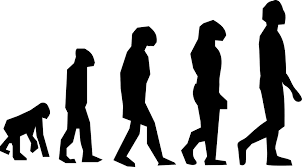
\includegraphics[width=\textwidth]{./images/fig1}


\end{frame}


\begin{frame}{Motivation \& General Principles}

	The \textbf{popularity} of GAs in the 80s and 90s was motivated by the following factors
	\bigskip

	\begin{enumerate}
		\item Evolution is known to be successful in nature, why not use its ideas within AI as well? 
		\item Back then they could search very complex hypothesis spaces
		\item They can be easily parallelized, therefore they can take advantage of powerful computer hardware
	\end{enumerate}


\end{frame}

\begin{frame}{Genetic Algorithms}
	\section{Genetic Algorithms}

	The \textbf{components} of a Genetic Algorithm are:
	
	\bigskip
	\centering

	i) A \textcolor{RoyalBlue}{learning problem} we wish to solve
	
	\bigskip

	\centering
	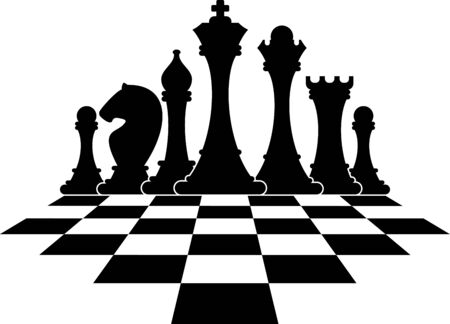
\includegraphics[width=4.5cm]{./images/fig2}

	\bigskip

	which allows us to define ii) a \textcolor{RoyalBlue}{fitness function} $f(x)$ 

\end{frame}


\begin{frame}{Genetic Algorithms}

	The \textbf{components} of a Genetic Algorithm are:
	
	\bigskip
	\centering

	iii) An \textcolor{RoyalBlue}{initial pool} of solutions e.g. programs that can play chess
	
	\bigskip

	\centering
	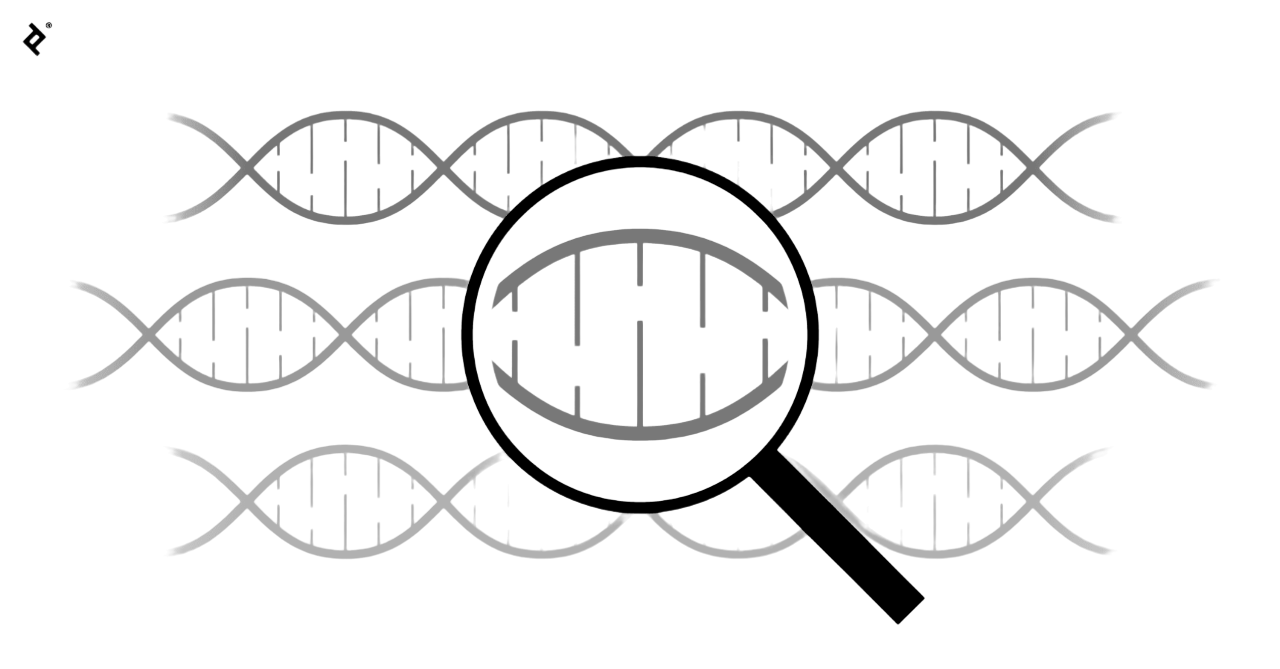
\includegraphics[width=8.5cm]{./images/fig3}

\end{frame}

\begin{frame}{Genetic Algorithms}

	The \textbf{components} of a Genetic Algorithm are:
	
	\bigskip
	\centering

	iv) An \textcolor{RoyalBlue}{evolution strategy}
	
	\bigskip
	That tells us how we should modify our initial pool of solutions based on how bad/well they perform on our aforementioned evaluation function $f(x)$

\end{frame}

\begin{frame}{Genetic Algorithms}

	A \textbf{Practical Example}: the \textcolor{RoyalBlue}{MAXONE Problem}
	\bigskip

	$\Rightarrow$ We have a string of 10 binary digits e.g. $1011010110$ and want to \textbf{maximize} the number of ones in a string.
	Our \textcolor{magenta}{objective}, therefore, becomes writing a program that automatically finds:
	\bigskip
	\begin{center}
		\textcolor{RoyalBlue}{\textbf{1111111111}}
	\end{center}

\end{frame}


\begin{frame}{Genetic Algorithms}

	A \textbf{Practical Example}: the \textcolor{RoyalBlue}{MAXONE Problem}
	\bigskip

	Let's start with a \textbf{randomly generated pool} of solutions $s$ which we call $G_1$ where G stays for Generation:


	\bigskip

	$G_1 = \begin{cases}
		s_0 = 0101100001     \\
		s_1 = 1100010001      \\
		s_2 = 1111110000	\\
		s_3 = 1010101111	\\ 
		s_4 = 0000000010	\\
	\end{cases}$

\end{frame}

\begin{frame}{Genetic Algorithms}

	A \textbf{Practical Example}: the \textcolor{RoyalBlue}{MAXONE Problem}
	\bigskip

	Let's now \textbf{evaluate} based on $f(x)$\footnote{We simply count how many ones appear in the string} how good/bad these solutions are

	\bigskip

	$G_1 = \begin{cases}
		s_0 = 0101100001  	 \\
		s_1 = 1100010001      \\
		s_2 = 1111110000	\\
		s_3 = 1010101111	\\ 
		s_4 = 0000000010	\\
	\end{cases}$

\end{frame}

\begin{frame}{Genetic Algorithms}

	A \textbf{Practical Example}: the \textcolor{RoyalBlue}{MAXONE Problem}
	\bigskip

	Let's now \textbf{evaluate} based on $f(x)$\footnote{We simply count how many ones appear in the string} how good/bad these solutions are

	\bigskip

	$G_1 = \begin{cases}
		s_0 = 0010100001 \rightarrow \textcolor{magenta}{\textbf{3}}	 \\
		s_1 = 1100010001 \rightarrow \textcolor{magenta}{\textbf{4}}     \\
		s_2 = 1111110000 \rightarrow \textcolor{magenta}{\textbf{6}} \\
		s_3 = 1110101111 \rightarrow \textcolor{magenta}{\textbf{8}} \\ 
		s_4 = 0000000010  \rightarrow \textcolor{magenta}{\textbf{1}} 	\\
	\end{cases}$

\end{frame}


\begin{frame}{Genetic Algorithms}

	A \textbf{Practical Example}: the \textcolor{RoyalBlue}{MAXONE Problem}
	\bigskip

	Let's now create a \textbf{new generation} $G_2$ where we start by only keeping the fittest solutions

	\bigskip

	$G_2 = \begin{cases}
		s_0 = 1110101111 \rightarrow \textcolor{magenta}{\textbf{8}} \\ 
		s_1 = 1111110000 \rightarrow \textcolor{magenta}{\textbf{6}} \\
		s_2 = 1100010001 \rightarrow \textcolor{magenta}{\textbf{4}}     \\
		s_3 = \(\cancel{0010100001}\) \rightarrow \textcolor{magenta}{\textbf{3}}	 \\
		s_4 = \(\cancel{0000000010}\)  \rightarrow \textcolor{magenta}{\textbf{1}} 	\\
	\end{cases}$

\end{frame}


\begin{frame}{Genetic Algorithms}

	A \textbf{Practical Example}: the \textcolor{RoyalBlue}{MAXONE Problem}
	\bigskip

	What to do with the spots which were taken by the worst solutions?

	\bigskip

	$G_2 = \begin{cases}
		s_0 = 110101111 \rightarrow \textcolor{magenta}{\textbf{8}} \\ 
		s_1 = 1111110000 \rightarrow \textcolor{magenta}{\textbf{6}} \\
		s_2 = 1100010001 \rightarrow \textcolor{magenta}{\textbf{4}}     \\
		s_3 = ?????????? \rightarrow \textcolor{magenta}{\textbf{?}}	 \\
		s_4 = ??????????  \rightarrow \textcolor{magenta}{\textbf{?}} 	\\
	\end{cases}$

\end{frame}	

\begin{frame}{Genetic Algorithms}

	A \textbf{Practical Example}: the \textcolor{RoyalBlue}{MAXONE Problem}
	\bigskip

	What to do with the spots which were taken by the worst solutions?

	\bigskip

	$\Rightarrow$ We can create two \textcolor{RoyalBlue}{new solutions} which take advantage of the two fittest solutions in $G_1$. We call them $c_1$ and $c_2$ were $c$ stays for child

	\bigskip

	\begin{centering}
		$c_1$ = \textcolor{green}{1110101111} + \textcolor{orange}{1111110000} = \textcolor{green}{11101} \textcolor{orange}{10000} \\
		$c_2$ = \textcolor{green}{1110101111} + \textcolor{orange}{1111110000} = \textcolor{green}{01111} \textcolor{orange}{111111}\\
	\end{centering}
\end{frame}


\begin{frame}{Genetic Algorithms}

	A \textbf{Practical Example}: the \textcolor{RoyalBlue}{MAXONE Problem}
	\bigskip

	What to do with the spots which were taken by the worst solutions?

	\bigskip

	$\Rightarrow$ We can create two \textcolor{RoyalBlue}{new solutions} which take advantage of the two fittest solutions in $G_1$. We call them $c_1$ and $c_2$ were $c$ stays for child

	\bigskip

	\begin{centering}
		$c_1$ = \textcolor{green}{11101\(\cancel{01111}\)} + \textcolor{orange}{\(\cancel{11111}\)10000} = \textcolor{green}{11101} \textcolor{orange}{10000} \\
		$c_2$ = \textcolor{green}{\(\cancel{11101}\)01111} + \textcolor{orange}{11111\(\cancel{10000}\)} = \textcolor{green}{01111} \textcolor{orange}{111111}\\
	\end{centering}
\end{frame}






\begin{frame}{Genetic Algorithms}

	A \textbf{Practical Example}: the \textcolor{RoyalBlue}{MAXONE Problem}
	\bigskip


	Let's evaluate the two new solutions ...

	\bigskip

	$G_2 = \begin{cases}
		s_0 = 1110101111 \rightarrow \textcolor{magenta}{\textbf{8}} \\ 
		s_1 = 1111110000 \rightarrow \textcolor{magenta}{\textbf{6}} \\
		s_2 = 1100010001 \rightarrow \textcolor{magenta}{\textbf{4}}     \\
		s_3 = \textcolor{green}{11101} \textcolor{orange}{10000}  \rightarrow \textcolor{magenta}{\textbf{?}}	 \\
		s_4 = \textcolor{green}{01111} \textcolor{orange}{11111}\  \rightarrow \textcolor{magenta}{\textbf{?}} 	\\
	\end{cases}$

\end{frame}



\begin{frame}{Genetic Algorithms}

	A \textbf{Practical Example}: the \textcolor{RoyalBlue}{MAXONE Problem}
	\bigskip

	\textbf{We have found a new best solution!}

	\bigskip

	$G_2 = \begin{cases}
		s_0 = 1110101111 \rightarrow \textcolor{magenta}{\textbf{8}} \\ 
		s_1 = 1111110000 \rightarrow \textcolor{magenta}{\textbf{6}} \\
		s_2 = 1100010001 \rightarrow \textcolor{magenta}{\textbf{4}}     \\
		s_3 = \textcolor{green}{11101} \textcolor{orange}{10000}  \rightarrow \textcolor{magenta}{\textbf{5}}	 \\
		s_4 = \textcolor{green}{01111} \textcolor{orange}{11111}\  \rightarrow \textcolor{magenta}{\textbf{9}} 	\\
	\end{cases}$

\end{frame}



\begin{frame}{Genetic Algorithms}

	A \textbf{Practical Example}: the \textcolor{RoyalBlue}{MAXONE Problem}
	\bigskip

	\textbf{We have found a new best solution!}

	\bigskip

	$G_2 = \begin{cases}
		s_0 = 1110101111 \rightarrow \textcolor{magenta}{\textbf{8}} \\ 
		s_1 = 1111110000 \rightarrow \textcolor{magenta}{\textbf{6}} \\
		s_2 = 1100010001 \rightarrow \textcolor{magenta}{\textbf{4}}     \\
		s_3 = \textcolor{green}{11101} \textcolor{orange}{10000}  \rightarrow \textcolor{magenta}{\textbf{5}}	 \\
		s_4 = \boxed{\textcolor{green}{01111} \textcolor{orange}{11111}\  \rightarrow \textcolor{magenta}{\textbf{9}}}\\
	\end{cases}$

\end{frame}


\begin{frame}{Genetic Algorithms}

	$\Rightarrow$ If we keep performing this iterative process, therefore creating many generations $G$, we will \textcolor{RoyalBlue}{eventually} find a solution that satisfies the MAXONE problem.  

\end{frame}

\begin{frame}{Genetic Algorithms}

	$\Rightarrow$ If we keep performing this iterative process, therefore creating many generations $G$, we will \textcolor{RoyalBlue}{eventually} find a solution that satisfies the MAXONE problem.  
    \bigskip
    \bigskip

    \begin{block}{\textbf{Elitism}}
   
        \textit{We ensure that the solution quality obtained by the GA will not decrease from one generation to the next, and that the best solutions of a generation will carry over to the next.}

    \end{block}

\end{frame}



\begin{frame}{Genetic Algorithms}



	\bigskip 

	For many real world problems this can take \textcolor{red}{prohibitively long} \Frowny{}

\end{frame}


\begin{frame}{Genetic Algorithms}

	In our MAXONE problem, we have simply removed the solutions within $G_1$ by ranking all the different solutions and discarding the last two ones.
	This was rather a simple heuristic.

	\bigskip

	$\Rightarrow$ Typically, in Genetic Algorithms a \textcolor{RoyalBlue}{probabilistic approach} decides whether to keep/discard a solution.

	\begin{centering}
		\begin{equation*}
			\text{Pr}(s_i) = \frac{f(s_i)}{\sum_{j=1}^{p} f(s_j)}
		\end{equation*}
	\end{centering}


\end{frame}


\begin{frame}{Genetic Algorithms}
	$\Rightarrow$ Next to the process that incrementally comes up with better and better \textit{solutions} and that, therefore, resembles \textcolor{RoyalBlue}{natural selection}, there's \textcolor{magenta}{one more} important component in Genetic Algorithms that mimics biological evolution
\end{frame}


\begin{frame}{Genetic Algorithms}
	$\Rightarrow$ The operations that recombine and mutate selected members of one specific generation $G$. We call these operations \textcolor{RoyalBlue}{\textbf{Genetic Operators}}

	\bigskip

	There are two operators which are the most common ones:
		\begin{itemize}
			\item \textit{Crossover} 
			\item \textit{Mutation}
		\end{itemize}

\end{frame}


\begin{frame}{Genetic Algorithms}

	\centering
	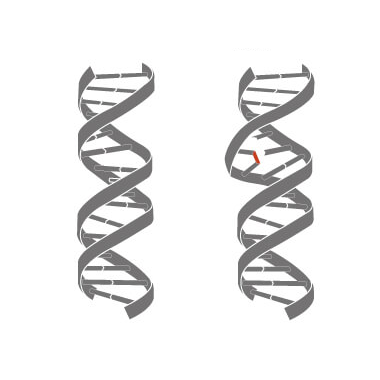
\includegraphics[width=8.5cm]{./images/fig4}

\end{frame}



\begin{frame}{Genetic Algorithms}
	
	$\Rightarrow$ Every \textit{Crossover} operator produces two new children $c_1$ and $c_2$ from two strings by copying selected bits from each parent $p$
	\biskip

	\begin{center}	
		\textcolor{RoyalBlue}{\textbf{Single-Point Crossover}}
	\end{center}

	\begin{align*}
		p_1 = 11101001000 \\ 
		p_2 = 00001010101
	\end{align*}

\end{frame}

\begin{frame}{Genetic Algorithms}
	
	$\Rightarrow$ Every \textit{Crossover} operator produces two new children $c_1$ and $c_2$ from two strings by copying selected bits from each parent $p$
	\biskip

	\begin{center}	
		\textcolor{RoyalBlue}{\textbf{Single-Point Crossover}}
	\end{center}

	\begin{align*}
		p_1 = \textcolor{green}{11101}001000 \\ 
		p_2 = 00001\textcolor{orange}{010101}
	\end{align*}

\end{frame}


\begin{frame}{Genetic Algorithms}
	
	$\Rightarrow$ Every \textit{Crossover} operator produces two new children $c_1$ and $c_2$ from two strings by copying selected bits from each parent $p$
	\biskip

	\begin{center}	
		\textcolor{RoyalBlue}{\textbf{Single-Point Crossover}}
	\end{center}

	\begin{align*}
		p_1 = \textcolor{green}{11101}001000 \\ 
		p_2 = 00001\textcolor{orange}{010101}
	\end{align*}
	\begin{align*}
		c_1 = \textcolor{green}{11101}\textcolor{orange}{010101} \\ 
	\end{align*}


\end{frame}

\begin{frame}{Genetic Algorithms}
	
	$\Rightarrow$ Every \textit{Crossover} operator produces two new children $c_1$ and $c_2$ from two strings by copying selected bits from each parent $p$
	\biskip

		\begin{center}	
		\textcolor{RoyalBlue}{\textbf{Single-Point Crossover}}
	\end{center}

	\begin{align*}
		p_1 = 11101\textcolor{green}{001000} \\ 
		p_2 = \textcolor{orange}{00001}010101
	\end{align*}
	\begin{align*}
		c_2 = \textcolor{orange}{00001}\textcolor{green}{001000} \\ 
	\end{align*}


\end{frame}


\begin{frame}{Genetic Algorithms}
	\begin{center}	
		\textcolor{RoyalBlue}{\textbf{Two-Point Crossover}}
	\end{center}
	
	\begin{align*}
		p_1 = 11101001000 \\ 
		p_2 = 00001010101
	\end{align*}
	

\end{frame}


\begin{frame}{Genetic Algorithms}
	\begin{center}	
		\textcolor{RoyalBlue}{\textbf{Two-Point Crossover}}
	\end{center}
	
	\begin{align*}
		p_1 = 11\textcolor{green}{10100}1000 \\ 
		p_2 = \textcolor{orange}{00}00101\textcolor{orange}{0101}
	\end{align*}
	

\end{frame}


\begin{frame}{Genetic Algorithms}
	\begin{center}	
		\textcolor{RoyalBlue}{\textbf{Two-Point Crossover}}
	\end{center}
	
	\begin{align*}
		p_1 = 11\textcolor{green}{10100}1000 \\ 
		p_2 = \textcolor{orange}{00}00101\textcolor{orange}{0101}
	\end{align*}
	\begin{align*}
		c_1 = \textcolor{orange}{00}\textcolor{green}{10100}\textcolor{orange}{0101}
	\end{align*}

\end{frame}


\begin{frame}{Genetic Algorithms}
	\begin{center}	
		\textcolor{RoyalBlue}{\textbf{Two-Point Crossover}}
	\end{center}
	
	\begin{align*}
		p_1 = \textcolor{green}{11}10100\textcolor{green}{1000} \\ 
		p_2 = 00\textcolor{orange}{00101}0101
	\end{align*}
	\begin{align*}
		c_2 = \textcolor{green}{11}\textcolor{orange}{00101}\textcolor{green}{1000}
	\end{align*}

\end{frame}


\begin{frame}{Genetic Algorithms}

	As you can imagine there are plenty of crossover combinations one can choose from. One could even design its own crossover operator but the \textit{single-point} and \textit{double-point} operators are typically good enough.

	\bigskip

	A special case of crossover which only requires a \textcolor{RoyalBlue}{single parent} is:
	\bigskip
	\begin{center}	
		\textcolor{RoyalBlue}{\textbf{Point Mutation}}
	\end{center}
	\begin{align*}
		p_1 = 11101001000
	\end{align*}
\end{frame}


\begin{frame}{Genetic Algorithms}

	As you can imagine there are plenty of crossover combinations one can choose from. One could even design its own crossover operator but the \textit{single-point} and \textit{double-point} operators are typically good enough.

	\bigskip

	A special case of crossover which only requires a \textcolor{RoyalBlue}{single parent} is:
	\bigskip
	\begin{center}	
		\textcolor{RoyalBlue}{\textbf{Point Mutation}}
	\end{center}
	\begin{align*}
		p_1 = 11101\textbf{0}1000
	\end{align*}
\end{frame}


\begin{frame}{Genetic Algorithms}

	As you can imagine there are plenty of crossover combinations one can choose from. One could even design its own crossover operator but the \textit{single-point} and \textit{double-point} operators are typically good enough.

	\bigskip

	A special case of crossover which only requires a \textcolor{RoyalBlue}{single parent} is:
	\bigskip
	\begin{center}	
		\textcolor{RoyalBlue}{\textbf{Point Mutation}}
	\end{center}
	\begin{align*}
		p_1 = 11101\textbf{1}1000
	\end{align*}
\end{frame}


\begin{frame}{Genetic Algorithms}

	As you can imagine there are plenty of crossover combinations one can choose from. One could even design its own crossover operator but the \textit{single-point} and \textit{double-point} operators are typically good enough.

	\bigskip

	A special case of crossover which only requires a \textcolor{RoyalBlue}{single parent} is:
	\bigskip
	\begin{center}	
		\textcolor{RoyalBlue}{\textbf{Point Mutation}}
	\end{center}
	\begin{align*}
		\mathbf{c_1} = 1110111000
	\end{align*}
\end{frame}


\begin{frame}{Genetic Programming}
	\section{Genetic Programming}


	\textcolor{RoyalBlue}{\textbf{Genetic Programming}} is a form of evolutionary computation in which the individuals in the evolving population are full \textcolor{magenta}{computer programs} rather than binary strings!

	\bigskip

	\begin{itemize}
		\item It is an extension of Genetic Algorithms
		\item Has demonstrated to produce intriguing results:
			\begin{enumerate}
				\item Design of electronic filter circuits
				\item Classification of segments of protein molecules
			\end{enumerate}
	\end{itemize}

	\bigskip

	
	$\Rightarrow$ How does it work?


\end{frame}


\begin{frame}{Genetic Programming}

	We need to find a way of representing a computer program. This is done via a \textcolor{RoyalBlue}{\textbf{tree}}:
		\begin{itemize}
			\item Each function call is represented by a node in the tree 
			\item The arguments of the function are given by the descendant nodes
		\end{itemize}

	\bigskip

	We would like to find a tree representation for the function
		\bigskip
		\begin{center}
		$\boxed{\mathbf{\text{sin}(x) + \sqrt{x^2+y}}}$
		\end{center}
\end{frame}



\begin{frame}{Genetic Programming}

	\bigskip
	$\Rightarrow$ Which should look like:

	\begin{center}
		$\boxed{\mathbf{\text{sin}(x) + \sqrt{x^2+y}}}$
		\end{center}

	\bigskip


	\Tree [.\circled{+} \qroof{\circled{x}}.\circled{sin} [.\circled{$\sqrt{}$} [.\circled{+} [.\circled{\textasciicircum} \circled{$x$} \circled{$2$} ] \circled{$y$} ] ] ]

\end{frame}


\begin{frame}{Genetic Programming}

	Let's consider the following two trees as candidate solutions:

	\begin{columns}[T] % align columns
	\begin{column}{.48\textwidth}
		\color{RoyalBlue}\rule{\linewidth}{4pt}

		\Tree [.\circled{+} \qroof{\circled{x}}.\circled{sin} [.\circled{\textasciicircum} [\circled{2} [.\circled{+} \circled{$x$} \circled{$y$} ]] ] ]

	
	\end{column}%
	\hfill%
	\begin{column}{.48\textwidth}
		\color{RoyalBlue}\rule{\linewidth}{4pt}

			\Tree [.\circled{+} \qroof{\circled{x}}.\circled{sin} [.\circled{$\sqrt{}$} [.\circled{+} [.\circled{\textasciicircum} \circled{$x$} \circled{$2$} ] \circled{$y$} ] ] ]


	\end{column}%
\end{columns}
\end{frame}



\begin{frame}{Genetic Programming}

	Let's consider the following two trees as candidate solutions:

	\begin{columns}[T] % align columns
	\begin{column}{.48\textwidth}
		\color{RoyalBlue}\rule{\linewidth}{4pt}

		\Tree [.\circled{+} \qroof{\circled{x}}.\circled{sin} [.\circled{\textasciicircum} [\circled{2} [.\textbf{\circled{\textcolor{red}{+}}} \circled{$x$} \circled{$y$} ]] ] ]

	
	\end{column}%
	\hfill%
	\begin{column}{.48\textwidth}
		\color{RoyalBlue}\rule{\linewidth}{4pt}

			\Tree [.\circled{+} \qroof{\circled{x}}.\circled{sin} [.\circled{$\sqrt{}$} [.\circled{+} [.\textbf{\circled{\textcolor{red}{\textasciicircum}}} \circled{$x$} \circled{$2$} ] \circled{$y$} ] ] ]


	\end{column}%
\end{columns}
\end{frame}



\begin{frame}{Genetic Programming}

	$\Rightarrow$ After performing a \textit{crossover} operation they will result in the following two new solutions:

	\begin{columns}[T] % align columns
	\begin{column}{.48\textwidth}
		\color{RoyalBlue}\rule{\linewidth}{4pt}

		\Tree [.\circled{+} \qroof{\circled{x}}.\circled{sin} [.\circled{\textasciicircum} [\circled{2} [.\textbf{\circled{\textcolor{red}{\textasciicircum}}} \circled{$x$} \circled{$2$} ]] ] ]

	
	\end{column}%
	\hfill%
	\begin{column}{.48\textwidth}
		\color{RoyalBlue}\rule{\linewidth}{4pt}

			\Tree [.\circled{+} \qroof{\circled{x}}.\circled{sin} [.\circled{$\sqrt{}$} [.\circled{+} [.\textbf{\circled{\textcolor{red}{+}}} \circled{$x$} \circled{$y$} ] \circled{$y$} ] ] ]


	\end{column}%
\end{columns}
\end{frame}


\begin{frame}{Genetic Programming}

	In Genetic Programming:
	\bigskip
	\begin{enumerate}
		\item We use the same genetic operators that define Genetic Algorithms
		\item However, we need to define the set of primitive functions e.g. $+,\sqrt{},\text{sin}...$ which is not trivial
		\item A solution is represented by an entire program tree, which can make their evaluation expensive
	\end{enumerate}

\end{frame}





\begin{frame}{Practical Applications}
	\section{Practical Applications}

	\centering
	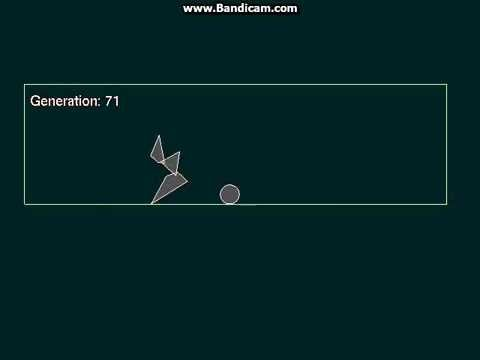
\includegraphics[width=6.5cm]{./images/ball}
	\url{https://www.youtube.com/watch?v=Gl3EjiVlz_4}


\end{frame}

\begin{frame}{Practical Applications}

	\centering
	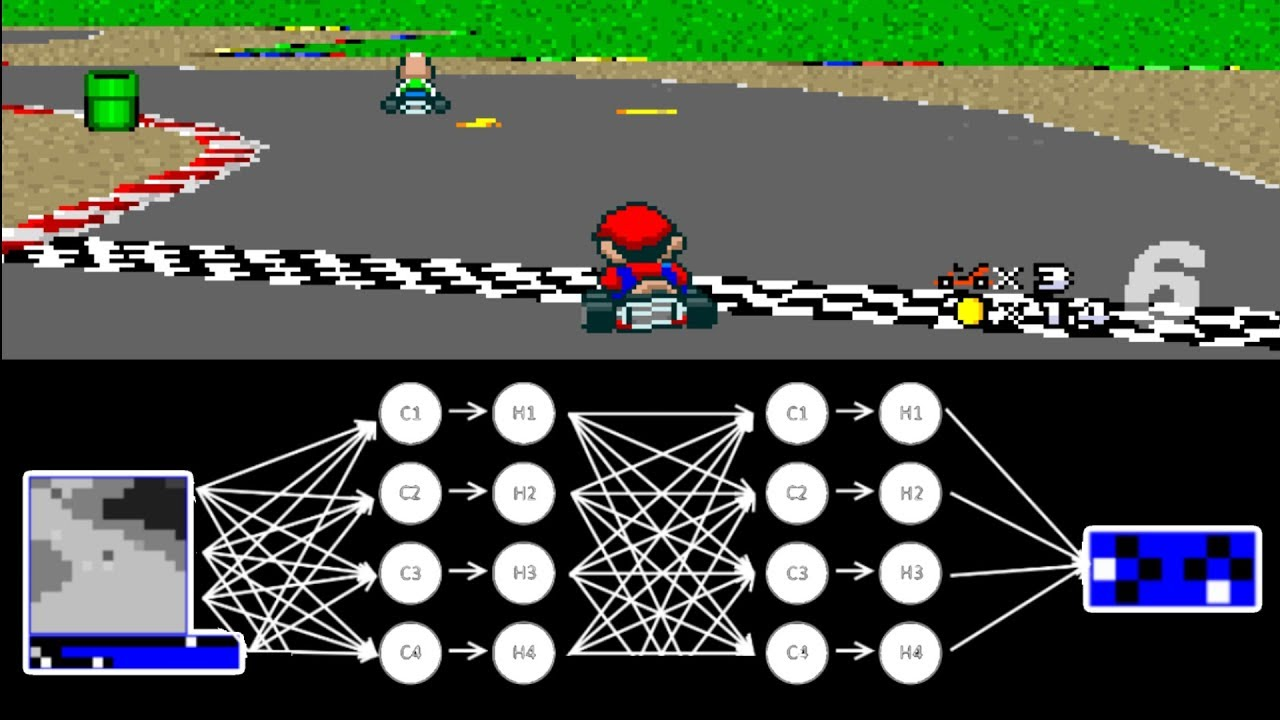
\includegraphics[width=8.cm]{./images/mario}

	\url{https://www.youtube.com/watch?v=qv6UVOQ0F44}

\end{frame}

\begin{frame}{Practical Applications}

	\centering
	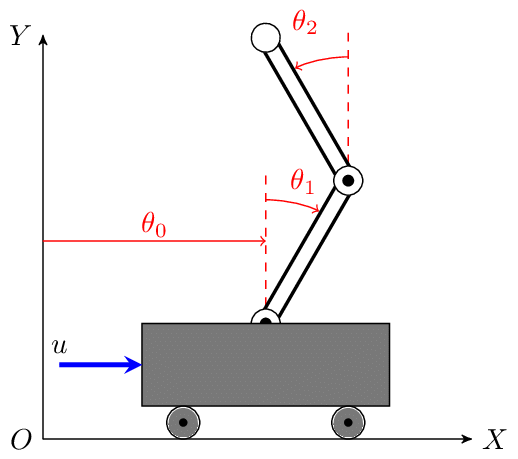
\includegraphics[width=7.cm]{./images/cartpole}

	\url{https://www.youtube.com/watch?v=czhhzKrBJfM}

\end{frame}

\begin{frame}{Practical Applications}

	\centering
	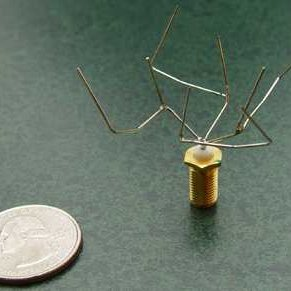
\includegraphics[width=6.5cm]{./images/antenna}

\end{frame}




\begin{frame}{Pros \& Cons of Genetic Algorithms}

	Among the main \textcolor{RoyalBlue}{benefits} we have that:

	\begin{itemize}
		\item The underlying concept is easy to understand $\textcolor{green}{\checkmark}$
		\item Can be used for multi-objective optimization $\textcolor{green}{\checkmark}$
		\item Support distributed learning $\textcolor{green}{\checkmark}$
		\item Same cooking recipe can be used across large variety of tasks $\textcolor{green}{\checkmark}$
		\item Work well when the problem is not differentiable $\textcolor{green}{\checkmark}$
	\end{itemize}

	
	\bigskip

	However there are some significant \textcolor{red}{limitations} as well ...
	

\end{frame}

\begin{frame}{Pros \& Cons of Genetic Algorithms}

	$\Rightarrow$ Among such limitations we have:
	\bigskip
	\begin{itemize}
		\item No convergence guarantees \textcolor{red}{\xmark}
		\item Computing the evaluation function $f(x)$ can be expensive \textcolor{red}{\xmark}
		\item Lots of implementation parameters need to be defined \textcolor{red}{\xmark}
		\item Termination Criteria? \textcolor{red}{\xmark}
	\end{itemize}

\end{frame}


\begin{frame}{Final References}

\begin{footnotesize}
	\begin{itemize}
		\item Mitchell, Tom M., and Tom M. Mitchell. Machine learning. Vol. 1. No. 9. New York: McGraw-hill, 1997. Chapter 9.
		\item Holland, John H. "Genetic algorithms." Scientific american 267.1 (1992): 66-73.
		\item Koza, John R., and Riccardo Poli. "Genetic programming." Search methodologies. Springer, Boston, MA, 2005. 127-164.
		\item B�ck, Thomas, and Hans-Paul Schwefel. "An overview of evolutionary algorithms for parameter optimization." Evolutionary computation 1.1 (1993): 1-23.
	\end{itemize}
\end{footnotesize}

\end{frame}


\begin{frame}{The GECCO Conference}

	\centering
	
\includegraphics[width=8.5cm]{./images/gecco}

\end{frame}



%============================================================================
\end{document}
